\documentclass[conference]{IEEEtran}
\usepackage[UTF8,scheme=plain,fontset=windows]{ctex}
\setmainfont{Times New Roman}
\usepackage{amsmath,amssymb}
\usepackage{booktabs,multirow}
\usepackage{siunitx}
\usepackage{graphicx}
\usepackage{xcolor}
\usepackage{tikz}
\usepackage{microtype}
\usepackage{stfloats}
\usetikzlibrary{arrows.meta,positioning,calc}
\usepackage[colorlinks=true,linkcolor=blue,citecolor=blue,urlcolor=blue]{hyperref}

\newcommand{\module}{WSR}
\definecolor{wsrblue}{HTML}{0072B2}
\definecolor{wsrorange}{HTML}{D55E00}
\tikzset{
  block/.style={draw,rounded corners=1.2pt,align=center,minimum height=5.5mm,minimum width=15mm,fill=blue!5},
  wave/.style={block,fill=orange!12,draw=wsrorange},
  sparse/.style={block,fill=blue!10,draw=wsrblue},
  sum/.style={circle,draw=black!70,fill=white,minimum size=4.5mm,inner sep=0pt,font=\small},
  flow/.style={-{Latex[length=1.7mm,width=1.1mm]},semithick,draw=black!75,rounded corners=1.5pt},
  waveflow/.style={flow,draw=wsrorange},
  sparseflow/.style={flow,draw=wsrblue},
  controlflow/.style={flow,draw=wsrorange,dashed},
  skipflow/.style={flow,draw=black!55,densely dotted},
  edgelabel/.style={font=\tiny,fill=white,inner sep=1pt,text=black!70}
}
\setlength{\textfloatsep}{6pt plus 2pt minus 2pt}
\setlength{\dbltextfloatsep}{6pt plus 2pt minus 2pt}
\setlength{\floatsep}{5pt plus 2pt minus 2pt}
\setlength{\intextsep}{5pt plus 2pt minus 2pt}
\setlength{\abovecaptionskip}{3pt}
\setlength{\belowcaptionskip}{0pt}
\renewcommand{\arraystretch}{0.94}
\sisetup{detect-all,group-separator={,},group-minimum-digits=4,uncertainty-mode=separate}
\renewcommand{\abstractname}{摘\ 要}
\renewcommand{\IEEEkeywordsname}{关键词}
\renewcommand{\figurename}{图}
\renewcommand{\tablename}{表}
\renewcommand{\refname}{参考文献}

\begin{document}

\title{WSR-YOLO：面向PCB缺陷检测的小波条件稀疏路由方法}
\author{
\IEEEauthorblockN{Jiefeng Liang\textsuperscript{a},
Lihua Luo\textsuperscript{a,b,*}, Sijin Tan\textsuperscript{a},
Yanni Lin\textsuperscript{a}, Zhizhuo Zhao\textsuperscript{a},
and Zhaofeng Cai\textsuperscript{a}}
\IEEEauthorblockA{\textsuperscript{a}Department of Computing, Guangdong University of Science and Technology, Dongguan 523083, China}
\IEEEauthorblockA{\textsuperscript{b}Faculty of Computer and Mathematical Sciences, Universiti Teknologi MARA, 40450 Shah Alam, Selangor, Malaysia}
\IEEEauthorblockA{\textsuperscript{*}Corresponding author: Lihua Luo, 260423630@qq.com}
\IEEEauthorblockA{项目仓库：\url{https://github.com/master-abc/WSR-YOLO}}
}
\maketitle

\begin{abstract}
算术稀疏性、具有信息性的特征路由、检测精度和部署效率常被视为可相互替代的证据。本文利用WSR分别审计这些命题；该精确预算模块以固定Haar响应对P3特征排序，仅优化得分最高的位置。在主要的DsPCBSD+测试集上，7组配对实验中WSR-YOLO11s的AP$_{50:95}$为46.69$\pm$0.72，YOLO11s为46.54$\pm$0.36，0.15点差异不显著（$p=0.8125$）。DeepPCB的3组描述性配对实验平均提高4.20点，但WSR在无缺陷模板上产生了更多报警。当预算为25\%时，两个数据集的路由在真实框内分别富集3.16倍和3.55倍；然而，空间先验解释了主要数据集的大部分富集现象，参数匹配卷积也复现了验证集增益。WSR仅增加1.33万参数和0.038 GFLOPs，但未融合的top-$k$与索引操作使推理时间达到基线的1.18--1.21倍。事后负样本感知训练将DeepPCB板级误报率从53.5\%降至27.5\%；改变输入约定的探索性成对参考检测器达到1.4\%误报率和0.959 F1。审计验证了非均匀、依赖图像的预算分配，却未发现可靠的WSR精度或系统优势。更一般地，结果表明工业检测中的路由重叠、名义FLOPs、仅正样本AP和组件归因需要分别设置对照。
\end{abstract}

\begin{IEEEkeywords}
PCB缺陷检测，稀疏路由，实证审计，小波，误报
\end{IEEEkeywords}

\fontsize{10}{12}\selectfont

\section{引言}
自动光学检测需要在重复走线与焊盘中定位尺寸小、对比度低的缺陷，同时避免在正常电路板上产生代价高昂的报警。稀疏或频率感知模块在该场景中看似具有吸引力，但四个命题容易被混淆：路由可以与缺陷重叠却不改善检测器；名义上的稀疏算子在硬件上可能更慢；仅正样本AP可能掩盖误报；精度变化也可能来自通用容量而非所提出的路由线索。因此，可信评估必须分别验证这些命题。

本文以小波条件稀疏路由（WSR）具体实现该评估。固定Haar响应提供方向细节与结构上下文，轻量路由器对P3位置排序，仅在$k=\operatorname{round}(\rho HW)$个令牌上执行通道变换。与将稠密变换结果乘以掩码不同，“聚合--优化--散射”真正缩小了该变换的空间计算范围。本文将WSR作为预算约束特征优化的受控探针，而不预设其能够提高精度或速度。

据此，本文将路由富集与同预算先验比较，在配对随机种子下评估检测性能，通过同一进程中顺序均衡的基准测试测量延迟，并在无缺陷输入上统计板级误报。随后利用组件对照和跨图像干预，检验有利诊断是否特异地来自所提出的小波条件路由。

\textbf{主要贡献如下：}（1）构建P3/8精确预算优化探针，使通道变换开销与$\rho$呈线性关系，并将该算术性质与实际速度明确区分；（2）将学习路由与随机、空间、激活、固定Haar及跨图像对照进行审计，再通过匹配卷积和融合对照检验组件归因；（3）在成对无缺陷模板上测量板级误报，揭示仅正样本PCB评估的盲点，并区分仅目标图像缓解方案与改变输入约定的参考辅助后续实验；（4）通过数据泄漏审计和配对随机种子协议，同时报告零效应、不利结果与正向诊断。主精度效应不显著，且所有验证变体均未通过精度--延迟联合门限；这些边界结果本身构成本文贡献，而不是被省略的失败案例。

\section{相关工作}
现代目标检测包括Faster R-CNN等候选区域方法~\cite{fasterrcnn}、FPN等多尺度特征金字塔结构~\cite{fpn}以及DETR等集合预测Transformer~\cite{detr}。Deformable DETR限制注意力采样位置~\cite{deformabledetr}，Sparse R-CNN则以学习得到的候选框替代稠密候选~\cite{sparsercnn}。这些稀疏形式针对注意力采样或目标查询；WSR保留原检测器，仅稀疏化一项高分辨率特征变换。作为同期背景，本文运行了固定版本的YOLOv10~\cite{yolov10}、YOLO11~\cite{yolo11}、YOLOv12~\cite{yolov12}、YOLO26~\cite{yolo26}、RT-DETRv2~\cite{rtdetrv2}、D-FINE~\cite{dfine}、DEIM~\cite{deim}和RF-DETR~\cite{rfdetr}官方实现。

不同PCB基准在采集方式和输入约定上存在实质差异。DeepPCB引入成对的无缺陷模板图像和对齐目标图像，并标注6类常见缺陷~\cite{deeppcb}；TDD-Net面向经数据增强扩展的六类PCB微小缺陷数据~\cite{tddnet}；DsPCBSD+则包含来自生产AOI图像的9类缺陷~\cite{dspcbsd}。PCB-YOLO~\cite{pcbyolo}、YOLO-HMC~\cite{yolohmc}、SRN-Net~\cite{srnnet}及近期基于Mamba的PCB-MMF~\cite{pcbmmf}分别通过注意力、上下文聚合、多尺度建模或轻量检测头改进PCB检测器，但其报告协议与本文并不等价。PCB-IND在当前协议冻结后发布，强调真实光照变化与自然长尾频率~\cite{pcbind}；它是尚未完成的重要外部基准，而不是本文现有证据。鉴于数据划分、输入约定和评估器并不一致，本文不将已发表的最高指标与受控实验直接合并比较。

频率感知网络以不同方式使用变换。WaveCNet利用小波抑制下采样混叠~\cite{wavecnet}，FcaNet将离散余弦分量映射为通道注意力~\cite{fcanet}，HWANet利用Haar特征进行遥感目标注意力建模~\cite{hwanet}，Wavelet-YOLO则结合空间域与频率域线索进行PCB检测~\cite{waveletyolo}。WSR的区别在于使用固定Haar响应对固定数量的特征单元排序，而不把单独的频率分支视为高效计算的证据。

条件计算涵盖空间自适应深度~\cite{sact}、稀疏块~\cite{sbnet}和离散空间门控~\cite{dynamicconv}。TokenLearner对自适应令牌进行池化~\cite{tokenlearner}，DynamicViT~\cite{dynamicvit}与EViT~\cite{evit}则剪枝或重组Transformer令牌。WSR为下游检测保留稠密P3网格，仅为通道MLP精确聚合$k$个位置并将结果散射回原位置。因此，本文重点不是提出通用稀疏分类体系，而是受控检验频率条件预算在微小缺陷检测器中是否有效、独特且快速。

\section{受审计的路由探针}
\subsection{小波条件路由}
设$\mathbf X\in\mathbb R^{C\times H\times W}$为P3/8特征。本文将其沿通道拆分为小波张量$\mathbf X_w$和优化张量$\mathbf X_r$，二者各含$C/2$个通道，从而避免稠密的$C\times C$投影。固定分组、步长为2的Haar卷积得到
\begin{equation}
(\mathbf{LL},\mathbf{LH},\mathbf{HL},\mathbf{HH})=\mathcal H(\mathbf X_w),
\end{equation}
其中使用可分离向量$[1,1]/\sqrt2$与$[-1,1]/\sqrt2$。将细节子带绝对值沿通道平均得到$E_{hf}$，保留$E_{ll}=\operatorname{mean}_c|\mathbf{LL}|$，并构造局部低频残差$G_{ll}=|E_{ll}-\operatorname{AvgPool}_{3\times3}(E_{ll})|$。上采样并按图像归一化后，小型卷积路由器预测
\begin{equation}
\mathbf S=R_\theta([\bar E_{hf};\bar E_{ll};\bar G_{ll}])
+\log(1+\bar E_{hf}+\bar G_{ll}).
\end{equation}
其中加性固定项提供有意义的初始排序。固定滤波器以不可训练的分组卷积缓冲区保存；若特征尺寸为奇数，则在下边界或右边界采用反射填充。$R_\theta$先用$3\times3$卷积将3种线索映射到16通道，再依次执行归一化、SiLU和$1\times1$投影。展平空间位置后，选择
\begin{equation}
\begin{aligned}
\mathcal I&=\operatorname{TopK}(\mathbf S,k),\\
k&=\min(HW,\max(4,\operatorname{round}(\rho HW))).
\end{aligned}
\end{equation}

\begin{figure*}[t]
\centering
\resizebox{0.88\textwidth}{!}{%
\begin{tikzpicture}[font=\scriptsize,node distance=3mm and 5mm]
  \node[block] (p3) {P3/8特征\\$\mathbf X$};
  \node[block,right=7mm of p3] (split) {通道拆分};
  \node[wave,above right=4mm and 9mm of split] (haar) {固定Haar线索\\+可学习小波门控};
  \node[wave,right=8mm of haar] (router) {稠密路由器\\得分$\mathbf S$};
  \node[sparse,below right=4mm and 9mm of split] (context) {共享$3{\times}3$\\上下文};
  \node[sparse,right=8mm of context] (topk) {top-$k$\\聚合};
  \node[sparse,right=8mm of topk] (mlp) {得分门控LN/MLP\\并散射回填};
  \node[block,right=10mm of mlp,yshift=8mm] (fuse) {softmax权重\\加权拼接};
  \node[sum,right=5mm of fuse] (add) {$+$};
  \node[block,right=5mm of add] (out) {输出\\$\mathbf Y$};
  \coordinate (waveleft) at ($(haar.north)+(0,4mm)$);
  \coordinate (waveright) at (fuse.north |- waveleft);
  \coordinate (sparseturn) at ($(mlp.east)+(4mm,0)$);
  \coordinate (skipleft) at ($(p3.south)+(0,-11mm)$);
  \coordinate (skipright) at (add.south |- skipleft);
  \draw[flow] (p3.east)--(split.west);
  \draw[waveflow] (split.north) |- (haar.west);
  \draw[sparseflow] (split.south) |- (context.west);
  \draw[controlflow] (haar.east)--(router.west);
  \draw[controlflow] (router.south)--node[edgelabel,right]{路由得分}(topk.north);
  \draw[sparseflow] (context.east)--(topk.west);
  \draw[sparseflow] (topk.east)--(mlp.west);
  \draw[waveflow] (haar.north)--(waveleft)--node[edgelabel,above]{小波门控}(waveright)--(fuse.north);
  \draw[sparseflow] (mlp.east)--(sparseturn)|-(fuse.west);
  \draw[skipflow] (p3.south)--(skipleft)--node[edgelabel,below]{恒等旁路}(skipright)--(add.south);
  \draw[flow] (fuse.east)--(add.west);
  \draw[flow] (add.east)--(out.west);
\end{tikzpicture}}
\caption{WSR紧凑流程。彩色实线表示分支特征流，橙色虚线表示路由与控制信号，灰色点线表示恒等旁路。固定Haar线索同时驱动可学习小波门控与稠密路由器，只有受得分门控的通道MLP使用精确的$\rho HW$预算。softmax分支权重由全局上下文、平均高频能量和选中路由置信度共同确定。}
\label{fig:wsr}
\end{figure*}

\subsection{稀疏优化与融合}
一个经softmax归一化的可学习$3\times3$卷积核在$\mathbf X_r$上提供稠密逐通道上下文，但仅聚合索引$\mathcal I$处的值。对于展平令牌$\mathbf T$与聚合上下文$\tilde{\mathbf T}_{\mathcal I}$，有
\begin{equation}
\mathbf T'_{\mathcal I}=\mathbf T_{\mathcal I}+\sigma(\mathbf S_{\mathcal I})\odot
\operatorname{MLP}\!\left(\operatorname{LN}(\mathbf T_{\mathcal I}+\gamma(\tilde{\mathbf T}_{\mathcal I}-\mathbf T_{\mathcal I}))\right).
\end{equation}
无偏置两层MLP的隐藏宽度为$\max(C/8,16)$；未路由令牌在分支融合前保持不变。上下文卷积核在通道间共享，通过softmax约束为非负且和为1，并采用复制填充。该设计避免构造稠密的unfold张量，同时保留聚合位置的局部信息。MLP复杂度从$O(HWC^2)$降为$O(\rho HWC^2)$，但$O(9HWC)$的上下文与路由操作仍是稠密的。硬索引无法获得梯度；路由器仅通过被选位置的置信因子和检测损失学习，不使用直通估计器或辅助路由损失。该梯度路径也促使本文设置固定路由器对照。

方向Haar幅值还生成sigmoid小波门$A_w$，从而有$\mathbf X'_w=\mathbf X_w\odot(1+A_w)$。双路softmax门利用全局上下文、平均高频能量和选定路由置信度融合两个分支：
\begin{equation}
\mathbf Y=\mathbf X+[\alpha_w\mathbf X'_w;\alpha_r\mathbf X'_r],
\qquad \alpha_w+\alpha_r=1.
\end{equation}
正式模型在P3处插入一个$\rho=0.25$的模块。后续保持恒等映射的变体融合近零初始化的分支增量，并以组归一化替换路由器中的批归一化；该变体仅用于锁定验证集后的工程迭代，从未替代正式测试模型。

\section{审计设计与实验}
\subsection{实验协议}
DsPCBSD+~\cite{dspcbsd}包含10,259幅图像、20,276个标注框和9个类别。其8,208幅训练图像被一次性划分为7,387幅训练图像和821幅验证图像；官方的2,051幅验证图像作为锁定测试集。DeepPCB~\cite{deeppcb}从官方训练部分取850/150幅图像，并使用全部500幅官方测试目标图像。正式检测仅使用目标图像，不使用配对模板。所有目标图像均为正样本，因此另行审计负样本板级行为。

\begin{table}[t]
\centering
\caption{转换与验证后冻结的数据划分。}
\label{tab:data}
\begingroup
\renewcommand{\arraystretch}{1.06}
\fontsize{7.5}{8.3}\selectfont
\setlength{\tabcolsep}{5pt}
\begin{tabular*}{\columnwidth}{@{\extracolsep{\fill}}llS[table-format=4.0]S[table-format=5.0]@{}}
\toprule
数据集 & 划分 & {图像} & {标注框} \\
\midrule
\multirow{3}{*}{DsPCBSD+} & 训练 & 7387 & 14590 \\
 & 验证 & 821 & 1594 \\
 & 锁定测试 & 2051 & 4092 \\
\addlinespace[1.5pt]
\multirow{3}{*}{DeepPCB} & 训练 & 850 & 5870 \\
 & 验证 & 150 & 1003 \\
 & 官方测试 & 500 & 3140 \\
\bottomrule
\end{tabular*}
\endgroup
\end{table}

训练前检查标注框范围、类别、空标签、重复伪标注框、文件路径、SHA-256内容哈希和感知相似度。感知相似度采用64位差值哈希，再计算灰度缩略图误差。表~\ref{tab:data}给出最终图像与标注框数量。跨划分精确重复数为0；保守筛查分别标记245对DsPCBSD+候选和14对DeepPCB候选。重复版图可能触发筛查，但缺少板号或批次标识，因此无法作出绝对无泄漏的断言。存在无效转换框或未按组随机划分的数据集不会被并入正式比较。

两种架构均从相同的预训练YOLO11s检查点开始，输入尺寸为640像素，最多训练80轮；DsPCBSD+使用7组配对随机种子，DeepPCB使用3组配对随机种子并仅作描述性分析。训练采用确定性SGD、余弦衰减、批量大小8、用于梯度累积的名义批量大小64、耐心值15的早停，以及相同的Mosaic计划。插入WSR会改变后续层索引，因此重映射预训练键；参数迁移率低于99\%的运行被拒绝。测试标签从不用于检查点或架构选择。预指定的P3/25\%候选首先必须通过三随机种子验证门限；比较器训练、组件对照和事后负样本研究具有独立的结果角色，不能在查看测试集后将该候选重新晋级。

所有方法均将原始检测结果导出到同一个固定版本COCO评估器~\cite{coco}。除AP$_{50:95}$外，还在结果JSON中保留AP$_{50}$、AP$_{75}$、分尺寸AP、AR和逐类别AP。本文报告均值$\pm$样本标准差、配对95\% $t$区间、精确双侧Wilcoxon检验以及跨数据集Holm校正。全量数据组件对照在验证集上使用3组配对随机种子，只作描述性分析，不作为经多重性校正的结论。批量为1的延迟在同一RTX 3090、同一进程中测量，采用12个交替ABBA/BAAB循环，每个模型和条件共获得600次同步观测。

\subsection{指标及证据角色}
对于图像$i$，设$M_i$为选中的路由单元，$B_i$为栅格化真实框单元的并集，$N_i=H_iW_i$。路由召回率$r_i=|M_i\cap B_i|/|B_i|$，富集度定义为
\begin{equation}
e_i=\frac{r_i}{|M_i|/N_i},
\end{equation}
随后对图像级数值取平均。因此，$e_i=1$表示同预算均匀期望，而非AP分数。若清洗后的模板上至少出现一个保留检测，则记为板级假阳性；板级误报率（board-FPR）为此类模板的比例，而每图FP数保留了警报数量信息。工作点召回率与F1采用类别匹配的IoU 0.5。主要终点仍是目标图像上的配对测试AP$_{50:95}$。路由指标与延迟检验机制和成本；逐类别、退化与频率切片仅作诊断；验证集组件对照和负样本感知阶段明确属于事后分析。该层级可防止有利的辅助结果替代不显著的主要比较。

\begin{figure}[!t]
\centering
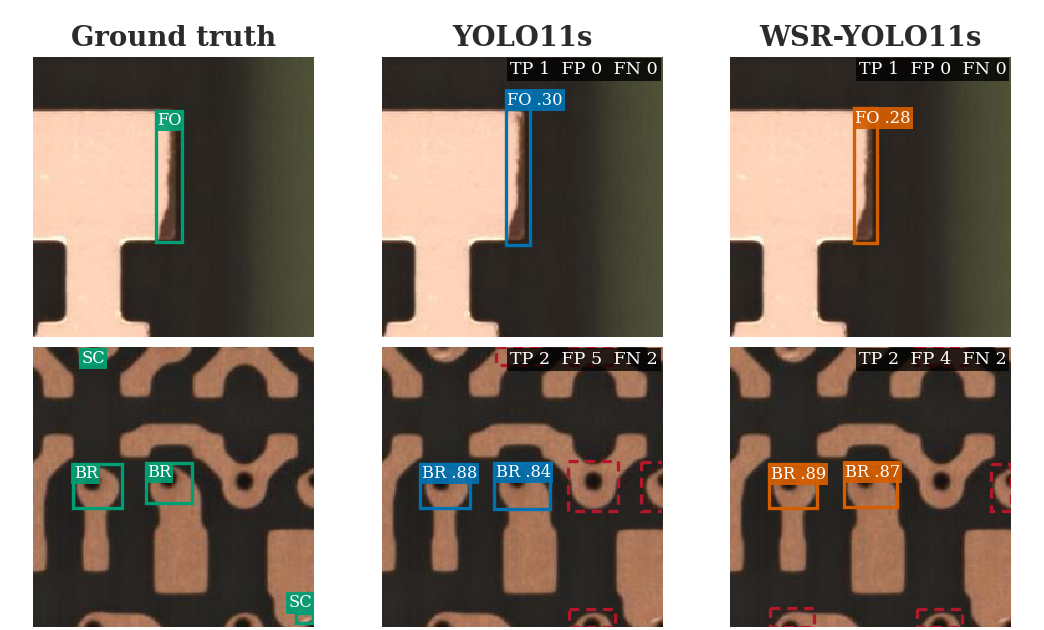
\includegraphics[width=\columnwidth]{figures/qualitative_operating_point.png}
\caption{采用验证集最大F1后处理的模型盲选DsPCBSD+示例。绿色表示真实框，蓝色/橙色表示真阳性，红色虚线表示假阳性。标签给出类别匹配IoU $\geq0.5$下的TP/FP/FN；FO、BR和SC分别表示基材异物、孔破和划痕。}
\label{fig:qualitative}
\end{figure}

\begin{figure*}[!b]
\centering
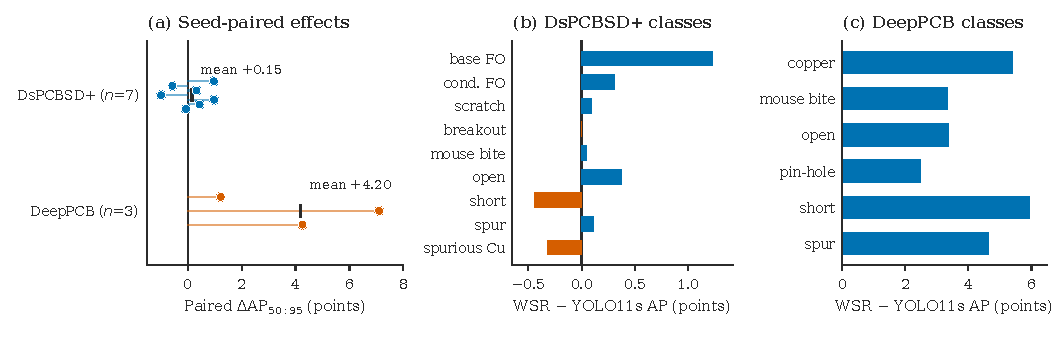
\includegraphics[width=0.89\textwidth]{figures/accuracy_evidence.pdf}
\caption{配对精度差异与逐类别精度差异。（a）圆点表示各配对随机种子，黑色短线及文字表示均值；（b--c）柱形表示逐类别平均差异，橙色表示性能下降。各切片相互依赖，属于诊断而非额外检验。}
\label{fig:accuracy_evidence}
\end{figure*}

\subsection{主要与描述性精度结果}
\begin{table}[!t]
\centering
\caption{架构受控的测试AP（\%），数值为均值$\pm$样本标准差。}
\label{tab:main}
\begingroup
\renewcommand{\arraystretch}{1.06}
\fontsize{7.5}{8.3}\selectfont
\setlength{\tabcolsep}{3.3pt}
\begin{tabular*}{\columnwidth}{@{\extracolsep{\fill}}llS[table-format=1.0]S[table-format=2.2(2)]S[table-format=2.2(2)]@{}}
\toprule
数据集 & 模型 & {$n$} & {AP$_{50:95}$} & {AP$_{50}$} \\
\midrule
\multirow{2}{*}{DsPCBSD+} & YOLO11s & 7 & 46.54 +- 0.36 & 80.25 +- 0.48 \\
 & WSR-YOLO11s & 7 & 46.69 +- 0.72 & 80.46 +- 0.86 \\
\addlinespace[1.5pt]
\multirow{2}{*}{DeepPCB} & YOLO11s & 3 & 64.61 +- 1.91 & 94.34 +- 1.07 \\
 & WSR-YOLO11s & 3 & 68.81 +- 4.12 & 95.46 +- 0.43 \\
\bottomrule
\end{tabular*}
\endgroup
\end{table}

在DsPCBSD+上，WSR在7个随机种子中的4个上胜出，但仅提升0.155 AP：$p=0.8125$，配对$d_z=0.207$，95\%差值区间为$[-0.535,0.844]$。DeepPCB的3次胜出带来4.196点增益，但精确检验仍为$p=0.25$（$p_{\mathrm{Holm}}=0.50$）。当$n=3$时，0.25也是双侧精确Wilcoxon检验能够取得的最小$p$值，因此即使3次一致胜出，该实验轨道也无法支持验证性显著结论。现有证据只支持依赖数据集的描述性效应。作为背景，固定版本的官方M尺度和Transformer实现在DsPCBSD+上达到49.44--53.08 AP，参数量为16.49--33.51M；WSR更紧凑，但并非当前最佳性能。

逐类别均值没有显示被总体统计掩盖的广泛提升：DsPCBSD+的9类中有7类上升，但其中5类变化不超过0.37点，另有2类下降。DeepPCB的6类均提升2.49--5.93点，但这些估计仅由3个随机种子支持。图~\ref{fig:qualitative}保持模型盲选的哈希顺序和真实类别覆盖，预测结果不参与图像选择。为便于观察工作点，该图使用各检查点在验证集上选定的分类阈值和重复框抑制，并显式给出TP/FP/FN数。该事后可视化不能替代统一协议下的AP比较。

\subsection{随机种子与误差分解}
图~\ref{fig:accuracy_evidence}(a)展示了汇总统计背后的配对观测。DsPCBSD+上的效应符号随随机种子改变，最大损失（$-0.99$）与最大增益（$+0.98$和$+0.97$）幅度相当，因此正均值并不意味着稳定提升。DeepPCB的3组配对均有利于WSR，但增益范围为1.22--7.11点。这种离散性加上$n=3$，使DeepPCB只能作为描述性而非验证性证据。

图~\ref{fig:accuracy_evidence}(b--c)给出相应的类别分解。在DsPCBSD+上，仅基材异物的提升超过1点，短路和多余铜箔下降；在DeepPCB上，所有类别均上升，其中短路和铜箔的变化最大。这些均值仍与相同随机种子耦合，不能解释为15项独立显著性检验。

按尺寸分层的诊断得到同样谨慎的结论。WSR使DsPCBSD+小/中/大目标AP分别变化$+0.54/-0.23/-4.23$点，使DeepPCB分别变化$+2.98/+4.53/-0.77$点；AR$_{100}$则分别变化$+0.18$和$+2.80$。大目标不是设计目标且样本可能稀少，因此这些未经校正的切片仅用于诊断。没有证据表明该模块能简单地改善所有尺度。

\subsection{同期检测器背景}
图~\ref{fig:context_route}(a)将小型受控模型与近期官方实现并列。所有比较器均使用相同的DsPCBSD+划分和COCO评估器，但保留与自身架构相适配的优化器和训练计划，因此该比较提供背景而非因果证据。所有较大模型均比WSR-YOLO11s高2.75--6.39 AP，同时参数量为其1.75$\times$--3.55$\times$。WSR较紧凑，但由于缺少完整的同设备延迟矩阵，现有证据既不支持最先进性能声明，也不支持速度排序。

\subsection{组件与路由审计}
预注册的30轮筛选并非事后选择最高均值行：预指定P3/25\%候选的三种子验证增益为1.283 AP、路由富集为2.469$\times$、种子13延迟比为0.982，在测试集仍未开启时满足声明门限，因此获准进入正式实验。表~\ref{tab:ablation}中更宽的35\%数据筛选仅提供背景：P3预算从5\%提高到25\%有帮助，稠密P3优化未进一步改善，而均值更高的P3+P4行未替代正式方案。全量数据审计中，普通参数匹配卷积与WSR相当，而等权融合和移除高频线索的均值更高。3轮锁定验证集的稳定性实验也未通过后续联合门限：$\Delta\mathrm{AP}\geq1.0$、富集$\geq2.0\times$且延迟$\leq1.20\times$。因此，验证趋势不能唯一归因于小波、学习路由或自适应融合。

全量数据审计在同一源代码提交和协议哈希下完成27项任务。WSR达到48.025 AP，重复基线为46.995 AP，但配对差值区间$[-0.158,2.219]$包含0。等权融合、无高频线索和参数匹配卷积分别达到48.314、48.296和48.057 AP。参数匹配卷积同样增加约13.1K参数，但增加0.176 GFLOPs；WSR则增加13.3K参数和0.038 GFLOPs。随机路由与固定Haar路由均低于完整WSR，仅尺度残差接近基线。这些结果保留了积极的验证趋势，却否定了简单的加性解释。

\begin{table}[t]
\centering
\caption{紧凑验证审计。筛选增益使用35\%训练子集；全量数据与稳定性行使用3个随机种子。}
\label{tab:ablation}
\begingroup
\renewcommand{\arraystretch}{1.04}
\fontsize{7.5}{8.3}\selectfont
\setlength{\tabcolsep}{3pt}
\begin{tabular*}{\columnwidth}{@{\extracolsep{\fill}}llS[table-format=+1.3]S[table-format=1.3]@{}}
\toprule
实验 & 变体 & {$\Delta$AP} & {延迟（$\times$）} \\
\midrule
\multirow{4}{*}{筛选} & P3/5\% & +0.273 & {\textemdash} \\
 & P3/25\% & +1.283 & {\textemdash} \\
 & P3/100\% & +1.185 & {\textemdash} \\
 & P3+P4/12.5\% & +1.486 & {\textemdash} \\
\addlinespace[1.5pt]
\multirow{4}{*}{全量数据} & WSR P3/25\% & +1.030 & {\textemdash} \\
 & 无高频线索 & +1.301 & {\textemdash} \\
 & 等权融合 & +1.319 & {\textemdash} \\
 & 匹配卷积 & +1.062 & {\textemdash} \\
\addlinespace[1.5pt]
\multirow{2}{*}{稳定性} & 最佳AP & +1.240 & 1.400 \\
 & 最佳$\leq1.20\times$ & +0.652 & 1.153 \\
\bottomrule
\end{tabular*}
\endgroup
\end{table}

在25\%预算下，学习路由对真实框单元的召回率分别为79.11\%和88.68\%，相对同预算随机选择的富集倍数为3.164$\times$和3.547$\times$。图~\ref{fig:context_route}(b)给出更强的对照。在DsPCBSD+上，中心先验和训练集占用先验接近学习路由（Holm校正$p=0.555$和$0.227$）；在DeepPCB上，学习路由超过所有对照。跨图像打乱显著降低富集，证明路由依赖图像，但不能证明这些信息导致精度变化。

标注框通过相同的letterbox几何变换并栅格化到路由网格。中心对照按到图像中心的距离排序，占用对照仅使用训练标签，激活/Haar对照使用当前输入但不使用学习得分；所有对照均精确选择$k$个单元。在64次跨图像置换中，DsPCBSD+的打乱富集为1.967$\times$ [1.964, 1.970]，DeepPCB为0.849$\times$ [0.844, 0.854]。稠密小波门的均值在框内并不更高，进一步限制了组件级因果解释。

\begin{figure*}[!t]
\centering
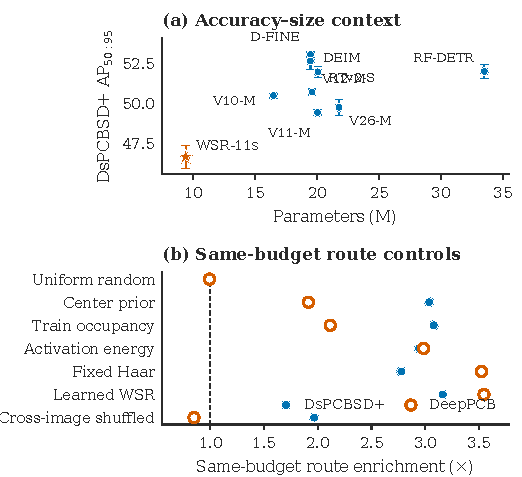
\includegraphics[width=0.87\textwidth]{figures/context_route_evidence.pdf}
\caption{模型规模与路由背景。（a）DsPCBSD+ AP与参数量（均值$\pm$标准差）；V10/V11/V12/V26为相应YOLO版本缩写。（b）同预算平均路由富集；虚线表示均匀期望，占用先验仅使用训练标签。}
\label{fig:context_route}
\end{figure*}

\begin{figure}[t]
\centering
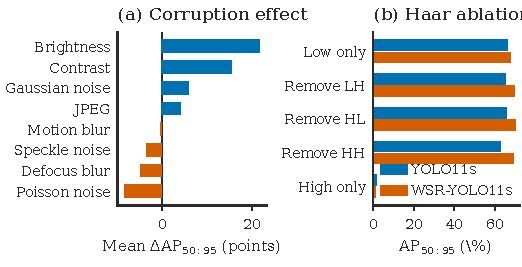
\includegraphics[width=\columnwidth]{figures/robustness_frequency_compact.pdf}
\caption{DeepPCB种子13诊断。（a）跨强度平均的WSR相对基线AP差，橙色表示负差异；（b）匹配输入Haar干预后的AP，分组柱形比较两个模型。}
\label{fig:robustness}
\end{figure}

WSR增加13,342个参数（0.14\%）和0.038 GFLOPs（0.18\%）。然而，在不同数据集及FP32/FP16条件下，仅模型延迟为基线的1.184$\times$--1.206$\times$，且每个配对循环区间均不包含1。稠密辅助操作以及未融合的top-$k$/索引主导了微小的算术节省，因此本文只声称稀疏通道计算，而不声称加速。

\begin{table}[t]
\centering
\caption{WSR/基线的配对仅模型延迟比及其95\%循环区间。}
\label{tab:latency}
\begingroup
\renewcommand{\arraystretch}{1.06}
\fontsize{7.5}{8.3}\selectfont
\setlength{\tabcolsep}{5pt}
\begin{tabular*}{\columnwidth}{@{\extracolsep{\fill}}lrr@{}}
\toprule
数据集 & FP32 & FP16 \\
\midrule
DsPCBSD+ & 1.184 [1.166, 1.203] & 1.194 [1.162, 1.227] \\
DeepPCB & 1.206 [1.193, 1.220] & 1.185 [1.166, 1.204] \\
\bottomrule
\end{tabular*}
\endgroup
\end{table}

\subsection{运行误报审计}
DeepPCB的500幅清洗模板揭示了仅正样本AP无法反映的失效模式。在置信度0.25下，种子13的WSR在56.6\%板上报警（每图1.472 FP），YOLO11s则为48.0\%（每图1.138 FP）；在审计的4个阈值上WSR均更差，如图~\ref{fig:false_alarm}(a)所示。3个事后、仅训练阶段的负样本感知步骤将三随机种子平均板级误报率从53.5\%降至27.5\%，同时保持0.946召回率，但接近1\%的阈值校准迁移效果较差。

置信度分别为0.05、0.10、0.25和0.50时，WSR板级误报率依次为87.6\%、77.0\%、56.6\%和35.0\%，种子13基线依次为79.0\%、66.2\%、48.0\%和28.0\%；配对板级和计数级检验在校正后仍显著。这些模板是对齐的参考裁剪，而非独立生产负样本，因此上述数值用于识别失效模式，不能估计部署误报率。

阶段1使用冻结的25\%训练模板子集作为空标签背景进行微调；阶段2使用全部850幅训练模板；阶段3对仅训练集内得分最高的四分之一模板进行过采样。训练计划在种子13上选定，随后冻结并用于种子42和3407。跨阶段的正样本AP从68.81升至72.44，固定阈值板级误报率从53.5\%降至27.5\%。验证集校准的1\%上限在测试集迁移后变为1.8\%--6.2\%误报率，同时平均召回率降至0.790，说明单纯提高阈值并不稳定。

\begin{figure}[!b]
\centering
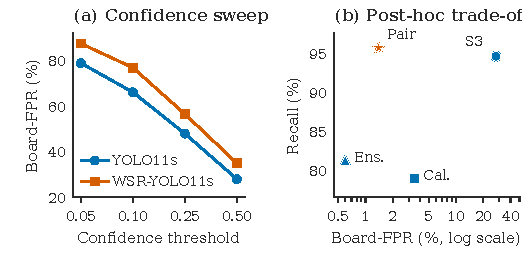
\includegraphics[width=\columnwidth]{figures/false_alarm_tradeoff.pdf}
\caption{DeepPCB负模板诊断。（a）仅目标图像的置信度扫描；（b）阶段3（S3）、校准阈值（Cal.）、三检查点共识（Ens.）与配对输入（Pair）的召回率--板级误报率权衡，横轴采用对数尺度。Pair改变了输入约定。}
\label{fig:false_alarm}
\end{figure}

共识方法需要3个检查点，且是在查看单模型测试结果后设计的。作为单次推理替代方案，设$c$和$r$分别为候选图像及光度对齐参考图像，以$d$表示二者经高斯平滑后的残差，则配对输入为
\begin{equation}
\begin{aligned}
s&=4\operatorname{sign}(d)\max(|d|-3,0),\\
I_{pair}&=\operatorname{clip}_{[0,255]}([c;\,c+s;\,c-s]).
\end{aligned}
\end{equation}
该形式对带符号变化进行颜色编码，同时仍向单个检测器提供候选图像外观。种子13使用合成负扰动进行适配；在生成r2重复实验前，检查点、类别阈值和小型结构变化掩码门均在正、负验证数据上选择。

锁定策略在r2上产生7/500次报警（精确95\%置信区间0.56\%--2.86\%），AP为72.63，F1为0.959。由于该方法族是在先前诊断之后提出的，改变了仅目标图像的输入约定，并扰动相同板模板，因此仍属于探索性结果。辅助的种子13退化实验显示，WSR/基线的干净归一化AP保持率分别为65.6\%和64.1\%；输入Haar重建确认低频结构至关重要，但两个单检查点研究均不能确定WSR内部小波分支的因果贡献。

\subsection{辅助鲁棒性与频率证据}
本文进一步在8类退化、每类5个严重度下评估DeepPCB种子13检查点。在40个配对条件中，WSR平均AP为46.51，YOLO11s为42.68，WSR在24个条件中胜出。增益并不均匀：主要集中在亮度、对比度、高斯噪声和JPEG压缩，而WSR在散焦模糊、泊松噪声和散斑噪声下更差，运动模糊下基本持平。按各检查点干净AP归一化后，保持率分别为65.6\%和64.1\%，因此结果只表明条件性鲁棒性，而非普遍鲁棒性。

频率实验对\emph{输入图像}实施单层Haar干预后重建，并评估未改变的检查点。仅低频重建下，WSR/基线AP为67.43/66.22；仅高频重建下为0.95/1.67。从输入中移除LH、HL或HH使WSR分别下降1.32、0.70和1.68点，使基线分别下降1.59、0.92和3.68点。这些观测表明低频结构仍然关键；由于干预位于网络之外且仅使用一个检查点，它不能证明WSR内部Haar分支导致精度差异，如图~\ref{fig:robustness}所示。

\section{研究发现、适用范围与局限性}
本审计区分出四项结论。第一，WSR确实以依赖图像的非均匀方式分配固定预算，但路由富集并不是精度替代指标：空间先验解释了主要数据集的大部分富集，匹配对照能够复现验证趋势，且7随机种子差值区间包含0。第二，算术稀疏性不等同于系统效率：被聚合位置上的MLP更便宜，但稠密辅助操作和不规则索引使实测模型反而更慢。第三，仅正样本AP遗漏了具有运行意义的失效模式；无缺陷模板改变了DeepPCB描述性AP增益给人的有利印象。第四，仅进行完整模块与基线的消融不足以完成组件归因，因为移除高频线索或自适应融合并未降低验证均值。

这些发现不局限于WSR。路由可视化应配合同预算空间对照，FLOPs应配合顺序均衡的同设备测量，仅正样本工业基准应增加负输入工作点，专用模块则应同时与匹配的通用容量和成熟即插即用注意力模块比较。最后一项比较在本文中尚未完成：受控实验轨道没有在相同P3插入位置和训练协议下纳入CBAM、CoordAtt、EMA或SimAM类模块。

最佳误报警折中来自参考辅助检测，而不是仅目标图像的WSR。共识结果与成对参考结果均为事后分析；后者仅使用一个随机种子、改变输入约定，并在已知模板的扰动上评估，而非独立生产板。其他局限包括DeepPCB仅有3组配对、仅使用一块GPU、较大模型缺少完整的同设备计时、组件对照仅用一个验证划分、硬top-$k$不连续，以及缺少板号/批次标识；相似度筛查留下的跨划分候选对也尚未解决。PCB-IND现已作为真实工业基准发布~\cite{pcbind}，但未在冻结协议下完成；后续研究应在训练或调参前声明其划分与假设。生产性结论还需要按模板、相机、光照和批次分层的锁定真实无缺陷板集合。

正式记录保留源代码、协议、数据集、检查点、预测和环境哈希。受控实验使用Python 3.10、PyTorch 2.5.1/CUDA 12.1和Ultralytics 8.4.50；比较器环境随结果一同保存。已验证的测试JSON被冻结，脚本可重建数据划分、验证组件实验从未评估测试集，并生成用于核对所有数值表格的机器可读汇总。这些材料支持数值复现，但不能替代在新电路板上的外部验证。代码与审计材料已公开于\url{https://github.com/master-abc/WSR-YOLO}；完整的归档发布还应保存冻结策略、原始预测以及可获取的检查点或权重哈希。数值可复现也不等同于推断独立：逐类别、尺寸、退化和阈值切片复用相同检查点与图像，因此本文将其视为分解而非额外样本；模型比较的抽样单位仍是配对随机种子，设备计时的单位则是交替循环。

\section{结论}
本文将WSR作为精确预算探针，发现框内路由富集、较低名义FLOPs、检测精度和部署表现并不会同步变化。WSR能够将选中的P3单元集中到缺陷框内，且只增加很少的算术开销，但既未建立可靠的主要精度增益，也未实现实际加速，其仅目标图像设置下的误报仍然较高。因此，本文的主要贡献是可审计的边界结果与评估模板，而不是WSR优越性声明。未来工作应在同一协议下测试成熟注意力对照、融合稀疏内核、更多配对随机种子、组安全PCB划分，并在独立生产负样本上进行预注册的参考辅助评估。

\IEEEtriggeratref{12}
\begin{thebibliography}{99}
\fontsize{7.8}{9.0}\selectfont
\setlength{\itemsep}{0pt}
\setlength{\parskip}{0pt}
\bibitem{fasterrcnn} S. Ren, K. He, R. Girshick, and J. Sun, ``Faster R-CNN: Towards Real-Time Object Detection with Region Proposal Networks,'' in \textit{NeurIPS}, 2015, pp. 91--99.
\bibitem{fpn} T.-Y. Lin et al., ``Feature Pyramid Networks for Object Detection,'' in \textit{CVPR}, 2017, pp. 2117--2125.
\bibitem{detr} N. Carion et al., ``End-to-End Object Detection with Transformers,'' in \textit{ECCV}, 2020, pp. 213--229.
\bibitem{deformabledetr} X. Zhu et al., ``Deformable DETR: Deformable Transformers for End-to-End Object Detection,'' in \textit{ICLR}, 2021.
\bibitem{sparsercnn} P. Sun et al., ``Sparse R-CNN: End-to-End Object Detection with Learnable Proposals,'' in \textit{CVPR}, 2021, pp. 14454--14463.
\bibitem{yolov10} A. Wang et al., ``YOLOv10: Real-Time End-to-End Object Detection,'' in \textit{NeurIPS}, vol. 37, pp. 107984--108011, 2024, doi: 10.52202/079017-3429.
\bibitem{yolo11} G. Jocher and J. Qiu, ``Ultralytics YOLO11,'' version 11.0.0, 2024. [Online]. Available: \url{https://github.com/ultralytics/ultralytics}
\bibitem{yolov12} Y. Tian, Q. Ye, and D. Doermann, ``YOLOv12: Attention-Centric Real-Time Object Detectors,'' in \textit{NeurIPS}, vol. 38, pp. 87151--87175, 2025, doi: 10.52202/085713-2627.
\bibitem{yolo26} G. Jocher, J. Qiu, M. Liu, S. Lyu, F. C. Akyon, and M. E. Kalfaoglu, ``Ultralytics YOLO26: Unified Real-Time End-to-End Vision Models,'' arXiv:2606.03748, 2026.
\bibitem{rtdetrv2} W. Lv et al., ``RT-DETRv2: Improved Baseline with Bag-of-Freebies for Real-Time Detection Transformer,'' arXiv:2407.17140, 2024.
\bibitem{dfine} Y. Peng et al., ``D-FINE: Redefine Regression Task of DETRs as Fine-Grained Distribution Refinement,'' in \textit{ICLR}, 2025.
\bibitem{deim} S. Huang et al., ``DEIM: DETR with Improved Matching for Fast Convergence,'' in \textit{CVPR}, 2025, pp. 15162--15171.
\bibitem{rfdetr} I. Robinson et al., ``RF-DETR: Neural Architecture Search for Real-Time Detection Transformers,'' in \textit{ICLR}, 2026, arXiv:2511.09554.
\bibitem{deeppcb} S. Tang, F. He, X. Huang, and J. Yang, ``Online PCB Defect Detector on a New PCB Defect Dataset,'' arXiv:1902.06197, 2019.
\bibitem{tddnet} R. Ding, L. Dai, G. Li, and H. Liu, ``TDD-Net: A Tiny Defect Detection Network for Printed Circuit Boards,'' \textit{CAAI Trans. Intell. Technol.}, vol. 4, no. 2, pp. 110--116, 2019, doi: 10.1049/trit.2019.0019.
\bibitem{dspcbsd} S. Lv et al., ``A Dataset for Deep Learning Based Detection of Printed Circuit Board Surface Defect,'' \textit{Scientific Data}, vol. 11, Art. no. 811, 2024, doi: 10.1038/s41597-024-03656-8.
\bibitem{pcbind} H. Yan, X. Yu, B. Ma, et al., ``Industrial Printed Circuit Board Surface Defect Dataset for Object Detection,'' \textit{Scientific Data}, 2026, doi: 10.1038/s41597-026-07684-4.
\bibitem{pcbyolo} J. Tang et al., ``PCB-YOLO: An Improved Detection Algorithm of PCB Surface Defects Based on YOLOv5,'' \textit{Sustainability}, vol. 15, no. 7, Art. no. 5963, 2023, doi: 10.3390/su15075963.
\bibitem{yolohmc} M. Yuan et al., ``YOLO-HMC: An Improved Method for PCB Surface Defect Detection,'' \textit{IEEE Trans. Instrum. Meas.}, vol. 73, Art. no. 2001611, pp. 1--11, 2024, doi: 10.1109/TIM.2024.3351241.
\bibitem{srnnet} L. Zhu and R. Zhao, ``A Novel PCB Surface Defect Detection Method Based on Separated Global Context Attention to Guide Residual Context Aggregation,'' \textit{Scientific Reports}, vol. 15, Art. no. 9620, 2025, doi: 10.1038/s41598-024-84961-5.
\bibitem{pcbmmf} L. Jin, Y. Feng, H. Yang, et al., ``A Multi-Cognitive PCB Defect Detection Model Integrating Mamba,'' \textit{Scientific Reports}, vol. 16, Art. no. 19124, 2026, doi: 10.1038/s41598-026-49734-2.
\bibitem{wavecnet} Q. Li, L. Shen, S. Guo, and Z. Lai, ``WaveCNet: Wavelet Integrated CNNs to Suppress Aliasing Effect for Noise-Robust Image Classification,'' \textit{IEEE Trans. Image Process.}, vol. 30, pp. 7074--7089, 2021, doi: 10.1109/TIP.2021.3101395.
\bibitem{fcanet} Z. Qin, P. Zhang, F. Wu, and X. Li, ``FcaNet: Frequency Channel Attention Networks,'' in \textit{ICCV}, 2021, pp. 783--792.
\bibitem{hwanet} B. Jin et al., ``HWANet: A Haar Wavelet-Based Attention Network for Remote Sensing Object Detection,'' \textit{PLOS ONE}, vol. 20, no. 9, Art. no. e0330759, 2025, doi: 10.1371/journal.pone.0330759.
\bibitem{waveletyolo} X. Zhong and K. Li, ``A PCB Bare Board Defects Detection Method Based on Dual-Domain Wavelet-YOLO,'' in \textit{Proc. 8th Int. Conf. Electron. Inf. Technol. Comput. Eng. (EITCE)}, 2024, pp. 1235--1240, doi: 10.1145/3711129.3711338.
\bibitem{sact} M. Figurnov et al., ``Spatially Adaptive Computation Time for Residual Networks,'' in \textit{CVPR}, 2017, pp. 1039--1048.
\bibitem{sbnet} M. Ren, A. Pokrovsky, B. Yang, and R. Urtasun, ``SBNet: Sparse Blocks Network for Fast Inference,'' in \textit{CVPR}, 2018, pp. 8711--8720.
\bibitem{dynamicconv} T. Verelst and T. Tuytelaars, ``Dynamic Convolutions: Exploiting Spatial Sparsity for Faster Inference,'' in \textit{CVPR}, 2020, pp. 2320--2329.
\bibitem{tokenlearner} M. S. Ryoo et al., ``TokenLearner: Adaptive Space-Time Tokenization for Videos,'' in \textit{NeurIPS}, 2021, pp. 12786--12797.
\bibitem{dynamicvit} Y. Rao et al., ``DynamicViT: Efficient Vision Transformers with Dynamic Token Sparsification,'' in \textit{NeurIPS}, 2021, pp. 13937--13949.
\bibitem{evit} Y. Liang et al., ``Not All Patches Are What You Need: Expediting Vision Transformers via Token Reorganizations,'' in \textit{ICLR}, 2022.
\bibitem{coco} T.-Y. Lin et al., ``Microsoft COCO: Common Objects in Context,'' in \textit{ECCV}, 2014, pp. 740--755.
\end{thebibliography}

\end{document}
